We let $\func{s}{x, y}$ describe the topography of the surface, 
$\func{h}{x,y,t}$ be the film thickness relative to $\func{s}{x,y}$ at any point in the $\lrp{x,y}$ plane at a time $t$, 
and $\func{\phi}{x,y,t} = \func{s}{x,y} + \func{h}{x,y,t}$ be the height of the free surface at any point in the $\lrp{x,y}$ plane at a time $t$.
We consider both the influence of gravity and acoustic streaming on the motion of the film, so 
our surface may also be inclined in addition to having Rayleigh surface acoustic waves (SAWs) propagating along the 
$x$-coordinate as shown in \cref{fig:diagram}. 

The starting point for modeling thin films are the incompressible Navier-Stokes equations 
\begin{gather}
    \nabla \cdot \vect{u} = 0
    \label{eq:incompress}\\
    \rho \lrp{\pderiv{\vecu}{t} + \lrp{\vecu \cdot \grad}\vecu} = -\grad p
    + \mu \grad^2 \vecu + \rho g \sin \beta \vect{i} - \rho g \cos \beta \vect{k}
    - \rho J e^{2k_i \lrp{x + \alpha_1 z}} \vect{i} - \rho J \alpha_1 e^{2k_i \lrp{x + \alpha_1 z}} \vect{k}
    \label{eq:ns-eq}
\end{gather}
where $\vect{u} = \lrp{u,v,w}$ is the fluid velocity, $p$ is the fluid pressure, $\rho$ is the fluid density, $\mu$ is the fluid viscosity
$k_i$ is the attenuation coefficient of the liquid, $\alpha_1$ is the geometric constant of the liquid, and $J = \lrp{1 + \alpha_1^2}A^2\omega^2 k_i$ 
is a constant we define to consolidate terms from acoustic streaming. We refer to see \cite{shiokawa1994saw} for more information on acoustic streaming 
and the derivation of the equations for acoustic forcing. 

\begin{figure}[ht]  
    \centering
    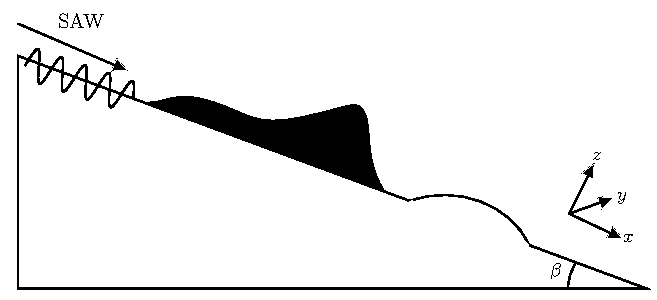
\includegraphics[width=.75\textwidth]{images/samp_diagram.pdf}
    \caption{A simplified sketch of a fluid flowing down a plane inclined at an angle $\beta$. The SAW travels
    from left to right, and the surface of the plane is described by a topography function $s$ that has a bump.}
    \label{fig:diagram}
\end{figure} 


\subsection{Lubrication Approximation}
As shown in \cite{kondic2003instabilities}, if the Reynold's number is sufficiently low, the inertial terms of the Navier-Stokes equations 
as well as the in plane derivatives and normal component of $\vecu$ can be ignored. Thus, under the effects of gravity and surface acoustic wave streaming forces, the lubrication approximation simplifies \cref{eq:ns-eq} to
\begin{gather}
    \grad_2 p = \mu \frac{\partial^2 \vect{v}}{\partial z^2} + \rho g \sin\beta \vect{i} - \rho J\cexpz\vect{i}
    \label{eq:pressure_grad}\\
    \pderiv{p}{z} = -\rho g \cos\beta - \rho J\alpha_1 \cexpz
    \label{eq:pressure_z}
\end{gather}
where $\grad_2 = \lrp{\partial_x, \partial_y}$ and 
$\vect{v} = \lrp{u, v}$. 

\subsection{Boundary Conditions}
The Laplace-Young boundary condition states that at the interface $z = \func{\phi}{x, y, t}$, the pressure is given by 
$\func{p}{\phi} = -\gamma \kappa + p_0$, where $\kappa$ is the curvature of the boundary, $\gamma$ is the surface tension, and $p_0$ is the atmospheric pressure. 
Thus, integrating \cref{eq:pressure_z} gives 
\begin{align}
    \nonumber \int_{\phi}^{z} \pderiv{p}{z} \; dz &=  \int_{\phi}^{z} -\rho g \cos \beta - \rho J\alpha_1 \cexpz \; dz\\
    \nonumber \func{p}{z} - \func{p}{\phi} &= -\lrp{z - \phi} \rho g \cos \beta - \frac{\rho J}{2k_i} \lrp{\cexpz - \cexpp}\\
    \func{p}{z} &= -\lrp{z - \phi}\rho g \cos \beta - \frac{\rho J}{2k_i} \lrp{\cexpz - \cexpp} -\gamma \kappa + p_0.  
    \label{eq:laplace_young}
\end{align}
If we define 
%\begin{align}
    $\func{P}{x, y, t} = \phi \rho g \cos\beta + \frac{\rho J}{2k_i} \cexpp - \gamma\kappa$, 
    %\label{eq:cap_P}
%\end{align}
this simplifies \cref{eq:laplace_young} to 
\begin{align*}
    \func{p}{z} = P - z\rho g \cos\beta - \frac{\rho J}{2k_i}\cexpz + p_0
\end{align*}
which further gives 
\begin{align}
    \grad_2 p %= \grad_2 \lrp{P - z\rho g \cos\beta - \frac{J}{2k_i}\cexpz + p_0}
    = \grad_2 \lrp{P - \frac{\rho J}{2k_i}\cexpz}
    = \grad P - \rho J\cexpz \vect{i}. 
    \label{eq:grad2_p_expanded}
\end{align}
Further boundary conditions include 
\begin{gather}
    \evalat{\vect{v}}{z = s\lrp{x,y}} = \vect{0} 
    \label{eq:bound_noslip}\\
    \evalat[\Big]{\pderiv{\vect{v}}{z}}{z = \phi\lrp{x,y,t}} = \vect{0} 
    \label{eq:bound_stress}
\end{gather}
where \cref{eq:bound_noslip} is a no-slip boundary condition along the surface $z = \func{s}{x,y}$ and \cref{eq:bound_stress}
enforces vanishing shear stresses along the fluid-air boundary $z = \func{\phi}{x,y,t}$. 

\subsection{Film Equation}
Using the Laplace-Young boundary condition and substituting \cref{eq:grad2_p_expanded} into \cref{eq:pressure_grad} yields 
\begin{align}
    \grad P = \mu \frac{\partial^2 \vect{v}}{\partial z^2} + \rho g \sin\beta \vect{i}. 
    \label{eq:pressure_grad_new}
\end{align}
Integrating \cref{eq:pressure_grad_new} twice with respect to $z$ and utilizing the boundary conditions in
\cref{eq:bound_noslip} and \cref{eq:bound_stress} gives
\begin{align}
    \nonumber \int_{s}^{z}\int_{z}^{\phi} \pderivtwo{\vect{v}}{z} \; dzdz &= \frac{1}{\mu}\int_{s}^{z}\int_{z}^{\phi} \lrp{\grad P - \rho g \sin\beta\vect{i}} \; dzdz \\
    %\nonumber \int_{s}^{z} \lrp{\evalat[\Big]{\pderiv{\vect{v}}{z}}{z = \phi} - \pderiv{\vect{v}}{z}} \; dz &= \frac{1}{\mu} \lrp{\grad P - \rho g \sin\beta\vect{i}} \int_{s}^{z}\lrp{\phi - z} \; dz\\
    \nonumber \int_{s}^{z} \pderiv{\vect{v}}{z} \; dz &= \frac{1}{\mu} \lrp{\grad P - \rho g \sin\beta\vect{i}} \int_{s}^{z} \lrp{z - \phi} \; dz\\
    %\nonumber \vect{v} - \evalat{\vect{v}}{z = s} &= \frac{1}{\mu} \lrp{\grad P - \rho g \sin\beta\vect{i}}  \lrp{\frac{z^2}{2} - \phi z} \Bigg|_{s}^z\\
    \vect{v} &=\frac{1}{\mu} \lrp{\grad P - \rho g \sin\beta\vect{i}} \lrp{\frac{z^2}{2} - \phi z - \frac{s^2}{2} + \phi s}. 
    \label{eq:vel_vectv}
\end{align}
Averaging over the height removes the $z$ dependence of $\vect{v} = \lrp{u, v}$ and gives the equation 
$\bar{\vect{v}} = \frac{1}{h} \int_{s}^{\phi} \vect{v} \; dz$.
Plugging in \cref{eq:vel_vectv} and solving this integral then gives 
\begin{align}
    \nonumber \bar{\vect{v}} &= \frac{1}{h} \int_{s}^{\phi} \frac{1}{\mu} \lrp{\grad P - \rho g \sin\beta\vect{i}} \lrp{\frac{z^2}{2} - \phi z - \frac{s^2}{2} + \phi s}  \; dz\\
    %\nonumber &= \frac{1}{\mu h} \lrp{\grad P - \rho g \sin\beta\vect{i}} \lrp{\frac{z^3}{6} - \frac{\phi z^2}{2} - z\lrp{\frac{s^2}{2} - \phi s}} \Bigg|_{s}^{\phi}\\
    \nonumber &= \frac{1}{\mu h} \lrp{\grad P - \rho g \sin\beta\vect{i}} \lrp{-\frac{\phi^3}{3} + \phi^2s - \phi s^2 + \frac{s^3}{3}}\\
    %\nonumber &=  \frac{1}{\mu h} \lrp{\grad P - \rho g \sin\beta\vect{i}} \lrp{-\frac{(h+s)^3}{3} + (h+s)^2s - (h+s) s^2 + \frac{s^3}{3}}\\
    &= -\frac{h^2}{3\mu} \lrp{\grad P - \rho g \sin\beta\vect{i}}.
    \label{eq:uv_bar}
\end{align}
The conservation of mass, when depth-averaged, gives 
$\pderiv{h}{t} + \grad \cdot \lrp{h\bar{\vect{v}}} = 0$
which results in 
\begin{align}
    \begin{aligned}
    \pderiv{h}{t} &= \frac{1}{3\mu} \grad \cdot \lrb{h^3 \lrp{\grad P - \rho g \sin \beta \vect{i}}}\\
    &= \frac{1}{3\mu} \grad \cdot \lrb{h^3 \lrp{\rho g \cos\beta \grad \phi - \gamma\grad\kappa - \rho g \sin \beta \vect{i} + \frac{\rho J}{2k_i}\grad \cexpp }}. 
    \end{aligned}
    \label{eq:thin_film_nokappa}
\end{align}
when plugging in \cref{eq:uv_bar}. Approximating the curvature $\kappa \approx \grad^2 \phi$ then gives 
\begin{align}
    \begin{aligned}
    \pderiv{h}{t} &= \frac{1}{3\mu} \grad \cdot \lrb{h^3 \lrp{\rho g \cos\beta \grad \phi - \gamma\grad\grad^2\phi - \rho g \sin \beta \vect{i} + \frac{\rho J}{2k_i}\grad \cexpp}}\\
    &= \frac{1}{3\mu} \lrb{ \grad \cdot \lrb{\rho g \cos \beta h^3 \grad \phi} - \grad \cdot \lrb{\gamma h^3 \grad\grad^2\phi} - \rho g \sin\beta \pderiv{h^3}{x} + \grad \cdot \lrb{\frac{\rho J}{2k_i}h^3\grad \cexpp}}.
    \end{aligned}
    \label{eq:thin_film_dim}
\end{align}

\subsection{Dimensionless Form}
We scale the in-plane coordinates and time by 
\begin{gather*}
    \bar{x} = \frac{x}{x_c}, \quad \bar{y} = \frac{y}{x_c}, \quad \bar{z} = \frac{z}{h_c}, \quad \bar{t} = \frac{t}{t_c}
    %\label{eq:coord_time_scales}
\end{gather*}
where an overline denotes a non-dimensional quantity. Substituting these scales 
into \cref{eq:thin_film_dim} and removing any overlines gives 
\begin{align}
    \begin{split}
        \frac{h_c}{t_c} \pderiv{h}{t} = &\frac{1}{3\mu} \lrb{
            \frac{h_c^4}{x_c^2} \rho g \cos \beta \grad \cdot \lrb{h^3\grad\phi} - 
            \frac{\gamma h_c^4}{x_c^4} \grad \cdot \lrb{h^3 \grad \grad^2 \phi} - 
            \frac{h_c^3}{x_c} \rho g \sin\beta \pderiv{h^3}{x}
        }\\
        &\qquad \qquad \qquad \qquad \qquad \qquad \qquad \qquad \qquad + \frac{1}{3\mu} \lrb{ 
            \frac{\rho J^* h_c^3}{2 x_c^2} \grad \cdot \lrb{h^3 \grad e^{2k_i \lrp{x + \alpha_1 \phi \lrp{h_c/x_c}}}}
        }
    \end{split}
    \label{eq:nondim_first}
\end{align}
where $J^* = \lrp{1+\alpha_1^2}A^2\omega^2$. 
By virtue of the fact that we are looking at thin films, we define $\varepsilon = h_c / x_c$ where $h_c \ll x_c$. 
This gives
%Additionally, by definition $\alpha_1 = -i \alpha$ where 
%\begin{equation*}
%    \alpha = \lrp{1 - \lrp{V_r/V_w}^2}^{1/2}
%\end{equation*}
%with $V_r$ and $V_w$ being the velocity of the SAW in the solid substrate and fluid, respectively. Since 
%$V_r > V_w$, 
%\begin{equation*} 
%    \alpha = i \lrp{\lrp{V_r/V_w}^2 - 1}^{1/2} \quad \rightarrow \quad \alpha_1 = \lrp{\lrp{V_r/V_w}^2 - 1}^{1/2}
%\end{equation*}
%is real and $\bigo{1}$. Thus, we can ignore any component of the exponent 
%that is multiplied by $\alpha_1$ and $\varepsilon$, which simplifies \cref{eq:nondim_first} to 
\begin{gather*}
    \nonumber \frac{h_c}{t_c} \pderiv{h}{t} = \frac{1}{3\mu} \lrb{
        \frac{h_c^4}{x_c^2} \rho g \cos \beta \grad \cdot \lrb{h^3\grad\phi} - 
        \frac{\gamma h_c^4}{x_c^4} \grad \cdot \lrb{h^3 \grad \grad^2 \phi} - 
        \frac{h_c^3}{x_c} \rho g \sin\beta \pderiv{h^3}{x} + 
        \frac{\rho J^* h_c^3}{2 x_c^2} \grad \cdot \lrb{h^3 \grad e^{2k_i \lrp{x + \alpha_1 \varepsilon \phi}}}
        %\frac{\eta h_c^5}{t_c^2 x_c^2} \pderiv{}{x} \lrb{h^3 \grad e^{2k_i x}}. 
    },
\end{gather*}
which can be further manipulated to the form 
\begin{align*}
    \pderiv{h}{t} = \frac{\gamma h_c^3 t_c}{3\mu x_c^4} \lrb{
        \frac{x_c^2 \rho g}{\gamma} \cos \beta \grad \cdot \lrb{h^3\grad\phi} - 
        \grad \cdot \lrb{h^3 \grad \grad^2 \phi} - 
        \frac{x_c^3 \rho g}{\gamma h_c} \sin\beta \pderiv{h^3}{x} + 
        \frac{\rho J^* x_c^2}{2 \gamma h_c} \grad \cdot \lrb{h^3 \grad e^{2k_i \lrp{x + \alpha_1 \varepsilon \phi}}}
    }.
    %\label{eq:nondim_sec}
\end{align*}
Choose $t_c$ such that 
\begin{align*}
    t_c = \frac{3\mu x_c^4}{\gamma h_c^3}.
    %\label{eq:x_and_t_scales}
\end{align*}
Additionally, we define the Bond number $\mathrm{Bo} = x_c^2 \rho g / \gamma$ and acoustic Weber number
$\mathrm{We_{ac}} = \rho \omega^2 A^2 x_c / \gamma$. 
Substituting these constants and expanding $J^*$ yields a final equation
\begin{align}
    \pderiv{h}{t} = \mathrm{Bo} \cos\beta \grad \cdot \lrb{ h^3 \grad \phi } - 
    \grad \cdot \lrb{h^3 \grad\grad^2\phi } - 
    \frac{\mathrm{Bo}}{\varepsilon} \sin\beta \pderiv{h^3}{x} + 
    \frac{\lrp{1 + \alpha_1^2} \mathrm{We_{ac}}}{2\varepsilon} \grad \cdot \lrb{h^3 \grad e^{2k_i \lrp{x + \alpha_1 \varepsilon \phi}}}. 
    \label{eq:nondim_final}
\end{align}   
The first term and third terms represent the out of plane and in plane influences of gravity, respectively, on 
the film while the second term represents the influence of capillary forces and the fourth term represents the 
contribution of SAW driving.  
 
\subsection{Two-Dimensional Equation and Enforcing a Film Front}
Although \cref{eq:nondim_final} is a simplified partial differential equation, 
it is still strongly nonlinear. To gain a basic understanding of some of its solutions,
we make the further simplification that the free surface of the thin film does not change
in the transverse direction (i.e.\! $h$ and $s$ are both $y$-independent). This assumption
further reduces our problem to only one variable in space and simplifies \cref{eq:nondim_final} to 
\begin{multline}
    \pderiv{h}{t} = \mathrm{Bo}\cos\beta \lrb{h^3 \phi_x}_x - \lrb{h^3 \phi_{xxx}}_{x} - \frac{\mathrm{Bo}}{\varepsilon} \sin\beta \lrb{h^3}_{x} \\ + 
    \frac{k_i \lrp{1 + \alpha_1^2}\mathrm{We_{ac}}}{\varepsilon} \lrb{h^3 e^{2k_i \lrp{x + \alpha_1 \varepsilon \phi}} \lrp{1 + \alpha_1 \varepsilon \phi_x}}_x
    \label{eq:two_dim_final}
\end{multline}
where $h$ and $\phi$ are now functions of $x$ and $t$.

Additionally, to enforce that the SAW forcing occurs starting from the film front, we redefine 
$k_i$ (in dimensionless form) as 
\begin{align}
    \func{k_i}{\phi} = x_c \lrp{\lrp{k_i^{\text{oil}} - k_i^{\text{air}}}\lrp{1 - e^{-x_c(\phi-b)/\lambda}} + k_i^{\text{air}}}
    \label{eq:k_i}
\end{align}
where $k_i^{\text{oil}}$ denotes the attenuation in the film and $k_i^{\text{air}}$ denotes the attenuation
outside the film. The $\lambda$ term is a dimensional constant that controls the steepness of the change from $k_i^{\text{air}}$ to $k_i^{\text{oil}}$, 
while $b$ denotes the precursor film height. In essence, when $h = b$, $k_i = x_c k_i^{\text{air}}$ and  
decays to $x_c k_i^{\text{oil}}$ as $h$ increases. See \cref{fig:attenuation} for an example of such a graph. 

\begin{figure}[ht]
    \centering
    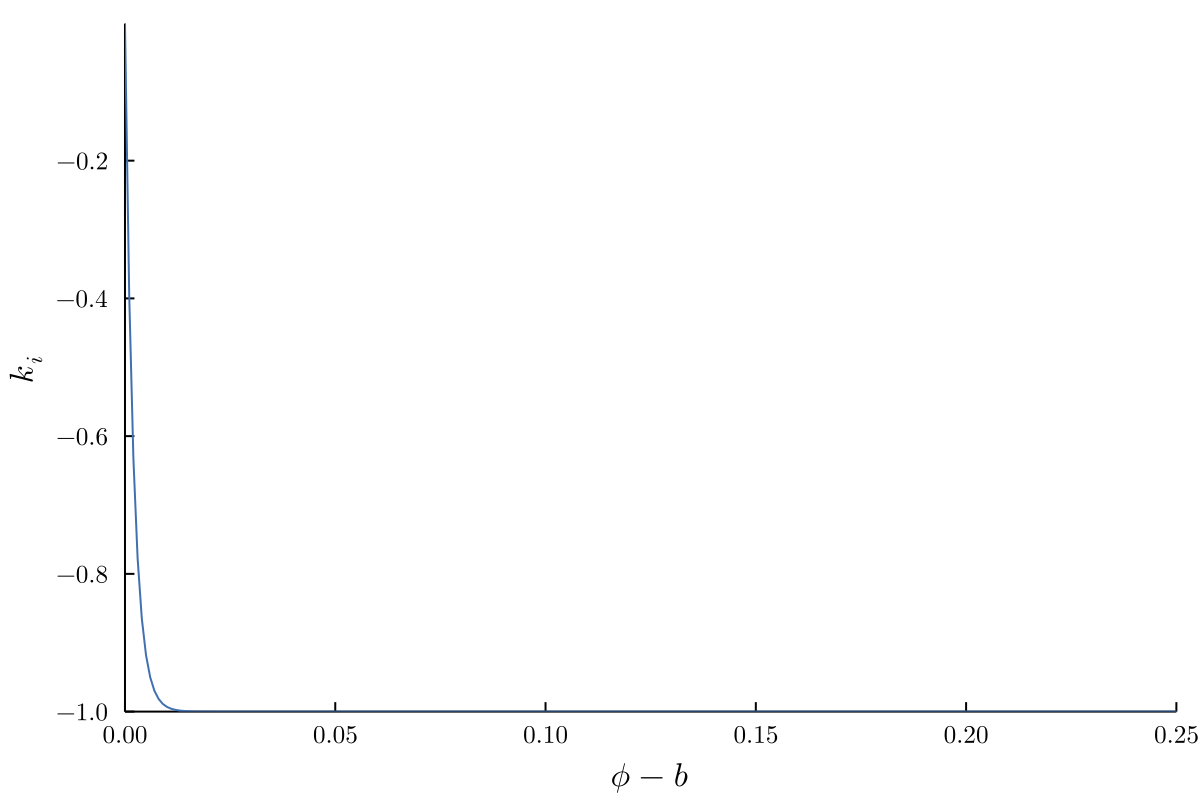
\includegraphics[scale=0.25]{images/attenuation.png}
    \caption{Attenuation as a function of $h$ for $k_i^{\text{oil}} = -1000 \lrb{m^{-1}}, k_i^{\text{air}} = -1 \lrb{m^{-1}}$, 
    $\lambda = 20*10^{-3} \lrb{m}$, and $x_c = 10^{-3}$.} 
    \label{fig:attenuation}
\end{figure}